\documentclass[
    alternativetitlepage=alternativ,
    cornerlogo=hgi_nds_logo2,
    sectionoverview,
]{rubpresentation}
\setbeamercovered{invisible}

\title[XML/JSON conversions]
{Bridging the Gap: Secure and lossless conversion\\ of XML data structures to the JSON format}
\subtitle{\small Bachelor thesis \hspace{3mm}{\scriptsize $\blacksquare$}\hspace{3mm} March 30, 2017 -- June 29, 2017}

\author[Holthuis]{Jan~Holthuis}

\institute[Advisors]
{%\inst{1}%
Advisors: Dennis Felsch \& Paul Rösler
}
\date{July 4, 2017}
\subject{Computer Science}

\titlegraphic{datacenter.jpg}
\sponsorlogo[height=7.6mm,interpolate=true]{hgi_nds_logo}

\definecolor{rubblue}{HTML}{003660}
\definecolor{rubgreen}{HTML}{8dae10}
\definecolor{rubgray}{HTML}{e7e7e7}

\usepackage{minted}
\usemintedstyle{rub}

\usepackage{tikzsymbols}
\setbeamercovered{invisible}

\begin{document}

\frame[plain]{\titlepage}

%\begin{frame}{The \texttt{\textbackslash note}-Macro}
%\begin{itemize}[<+->]
%\item normal text for the presentation.
%\note<1-2>[item]{Say something to the audience!}
%\item and text for the presentation.
%\item foo
%\end{itemize}
%\note<2>{Another note for you!}
%\end{frame}

%\note[enumerate]{\item foo \item bar \item baz \item foobar}

\section{Introduction}

\begin{frame}
  \frametitle{}
  \framesubtitle{}
\end{frame}

\section{Approach}

\begin{frame}
  \frametitle{Finding a lossless/secure method}
  \framesubtitle{}
  \begin{itemize}
    \item{} Define verifiable criteria for lossless conversion
    \item{} Check available conversion tools
    \item{} If no sufficient solution exists:
      \begin{itemize}
        \item{} Develop custom solution or extend existing one
      \end{itemize}
  \end{itemize}
\end{frame}

\begingroup
  \setbeamercolor{background canvas}{bg=white}
  \begin{frame}[fragile]
    \vspace{-1cm}
    \begin{center}
      \includestandalone[height=0.9\textheight]{thesis/flowchart_conversiontest}
    \end{center}
  \end{frame}
\endgroup

\begingroup
  \setbeamercolor{background canvas}{bg=white}
  \begin{frame}[fragile]
    \vspace{-1cm}
    \begin{center}
      \includestandalone[height=0.9\textheight]{thesis/flowchart_securitytest}
    \end{center}
  \end{frame}
\endgroup

\begin{frame}
  \frametitle{Converters tested}
  \framesubtitle{}
  \begin{itemize}
    \item{} \textbf{Cobra vs Mongoose} Paul Battley, MIT, Ruby
    \item{} \textbf{GreenCape XML Converter} Niels Braczek, MIT, PHP
    \item{} \textbf{Json-lib} Andres Almiray, Apache~2.0, Java
    \item{} \textbf{JsonML} Stephen M. McKamey, MIT, JavaScript
    \item{} \textbf{JXON} Martin Raifer, Mozilla, GNU GPL~3.0, JavaScript
    \item{} \textbf{Json.NET} James Newton-King, MIT, C\#
    \item{} \textbf{org.json.XML} Sean Leary / JSON.org, MIT, Java
    \item{} \textbf{Pesterfish} Jacob Smullya, MIT, Python
    \item{} \textbf{x2js} Abdulla G. Abdurakhmanov, Apache~2.0, JavaScript
    \item{} \textbf{x2js (Fork)} Sander Saares / Axinom, Apache~2.0, JavaScript
    \item{} \textbf{xmljson} S. Anand, MIT, Python
  \end{itemize}
\end{frame}

\section{Evaluation}

\begin{frame}
  \frametitle{Test results}
  \framesubtitle{}
  \begin{itemize}
    \item{} Tested 11 converters
    \item{} Some support multiple modes
    \item{} Used 123 test documents
    \item[$\Rightarrow$]{} more than 2000 (!) tests
  \end{itemize}
\end{frame}

\subsection{General XML support}

\begingroup
  \setbeamercolor{background canvas}{bg=white}
  \begin{frame}[fragile]
    \vspace{-1.15cm}
    \begin{center}
      \includestandalone[width=0.8\textwidth]{thesis/resulttable-basic}
    \end{center}
  \end{frame}
\endgroup

\begin{frame}
  \frametitle{General XML support}
  \framesubtitle{}
  \begin{itemize}
    \item{} Mixed Content support is sketchy
    \item{} Leading/Trailing Whitespace and indentation is often discarded
    \item{} Only few converters support Element Order
    \item{} Processing Instructions are not supported at all
  \end{itemize}
\end{frame}

\subsection{Character Support}

\begin{frame}
  \frametitle{Character Support}
  \framesubtitle{Whitespace}
  \begin{itemize}
    \item{} Some converters discard leading/trailing Whitespace
    \item{} Can affect not only Tab, Carriage Return, Line Feed and Space\dots{}
    \item{} \dots{}but lots of other chars, too!
    \begingroup
      \footnotesize
      \begin{columns}
        \begin{column}{0.5\textwidth}
          \begin{center}
            \begin{tabular}{lr}
              \texttt{CHARACTER TABULATION}               & \texttt{000009}\\
              \texttt{LINE FEED (LF)}                     & \texttt{00000A}\\
              \texttt{CARRIAGE RETURN (CR)}               & \texttt{00000D}\\
              \texttt{SPACE}                              & \texttt{000020}\\
              \texttt{NEXT LINE (NEL)}                    & \texttt{U+0085}\\
              \texttt{NO-BREAK SPACE}                     & \texttt{U+00A0}\\
              \texttt{OGHAM SPACE MARK}                   & \texttt{U+1680}\\
              \texttt{MONGOLIAN VOWEL SEPARATOR}          & \texttt{U+180E}\\
              \texttt{EN QUAD}                            & \texttt{U+2000}\\
              \texttt{EM QUAD}                            & \texttt{U+2001}\\
              \texttt{EN SPACE}                           & \texttt{U+2002}\\
              \texttt{EM SPACE}                           & \texttt{U+2003}\\
              \texttt{THREE-PER-EM SPACE}                 & \texttt{U+2004}\\
            \end{tabular}
          \end{center}
        \end{column}
        \begin{column}{0.5\textwidth}
          \begin{center}
            \begin{tabular}{lr}
              \texttt{FOUR-PER-EM SPACE}                  & \texttt{U+2005}\\
              \texttt{SIX-PER-EM SPACE}                   & \texttt{U+2006}\\
              \texttt{FIGURE SPACE}                       & \texttt{U+2007}\\
              \texttt{PUNCTUATION SPACE}                  & \texttt{U+2008}\\
              \texttt{THIN SPACE}                         & \texttt{U+2009}\\
              \texttt{HAIR SPACE}                         & \texttt{U+200A}\\
              \texttt{LINE SEPARATOR}                     & \texttt{U+2028}\\
              \texttt{PARAGRAPH SEPARATOR}                & \texttt{U+2029}\\
              \texttt{NARROW NO-BREAK SPACE}              & \texttt{U+202F}\\
              \texttt{MEDIUM MATHEMATICAL SPACE}          & \texttt{U+205F}\\
              \texttt{IDEOGRAPHIC SPACE}                  & \texttt{U+3000}\\
              \texttt{ZERO WIDTH NO-BREAK SPACE}          & \texttt{U+FEFF}\\
            \end{tabular}
          \end{center}
        \end{column}
      \end{columns}
    \endgroup
  \end{itemize}
\end{frame}

\begin{frame}
  \frametitle{Character Support}
  \framesubtitle{What's this?}
  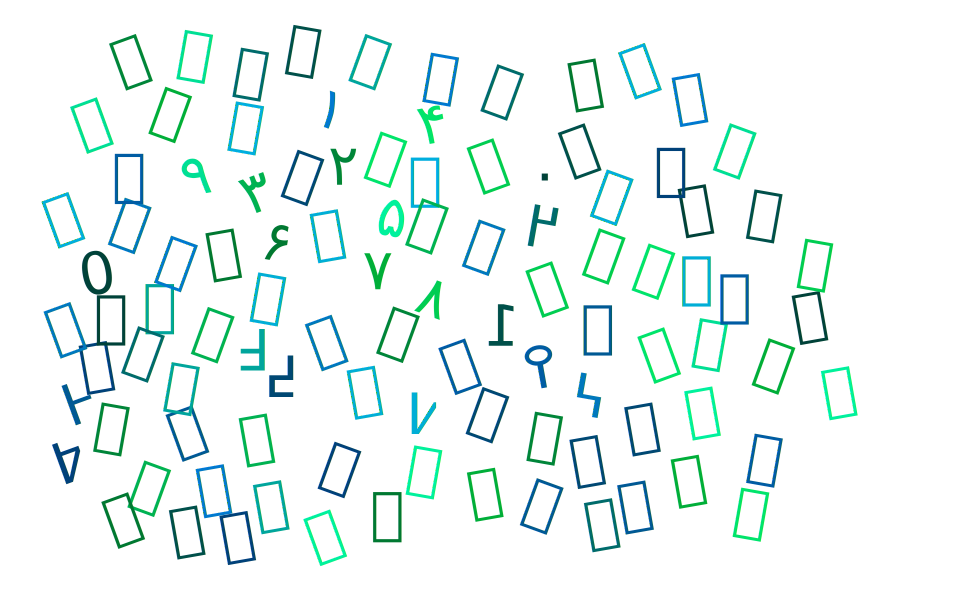
\includegraphics[width=\textwidth]{letternumerals}
  \visible<2->{%
    \begin{tikzpicture}[remember picture,overlay]%
      \node[draw=none,fill=white,font=\Huge,inner sep=5mm,rounded corners=10mm] at (current page.center) {Numerals!};%
    \end{tikzpicture}%
  }
\end{frame}

\begin{frame}
  \frametitle{Character Support}
  \framesubtitle{Numeral Transformation}
  \begin{itemize}
    \item{} \textbf{xmljson} transforms Unicode numerals into their ASCII equivalents
    \item{} \dots{}but only those on the Unicode BMP plane (U+000000 to U+00FFFF)
      \begingroup
      \tiny
  \begin{columns}
    \begin{column}{0.5\textwidth}
      \begin{center}
      \begin{tabular}{lrr}
\texttt{ARABIC-INDIC DIGITS} & \texttt{U+0669} & \texttt{U+0660}\\
\texttt{EXTENDED ARABIC-INDIC DIGITS} & \texttt{U+06F9} &  \texttt{U+06F0}\\
\texttt{NKO DIGITS} & \texttt{U+07C9} &  \texttt{U+07C0}\\
\texttt{DEVANAGARI DIGITS} & \texttt{U+096F} &  \texttt{U+0966}\\
\texttt{BENGALI DIGITS} & \texttt{U+09EF} &  \texttt{U+09E6}\\
\texttt{GURMUKHI DIGITS} & \texttt{U+0A6F} &  \texttt{U+0A66}\\
\texttt{GUJARATI DIGITS} & \texttt{U+0AEF} &  \texttt{U+0AE6}\\
\texttt{ORIYA DIGITS} & \texttt{U+0B6F} &  \texttt{U+0B66}\\
\texttt{TAMIL DIGITS} & \texttt{U+0BEF} &  \texttt{U+0BE6}\\
\texttt{TELUGU DIGITS} & \texttt{U+0C6F} &  \texttt{U+0C66}\\
\texttt{KANNADA DIGITS} & \texttt{U+0CEF} &  \texttt{U+0CE6}\\
\texttt{MALAYALAM DIGITS} & \texttt{U+0D6F} &  \texttt{U+0D66}\\
\texttt{SINHALA LITH DIGITS} & \texttt{U+0DEF} &  \texttt{U+0DE6}\\
\texttt{THAI DIGITS} & \texttt{U+0E59} &  \texttt{U+0E50}\\
\texttt{LAO DIGITS} & \texttt{U+0ED9} &  \texttt{U+0ED0}\\
\texttt{TIBETAN DIGITS} & \texttt{U+0F29} &  \texttt{U+0F20}\\
\texttt{MYANMAR DIGITS} & \texttt{U+1049} &  \texttt{U+1040}\\
\texttt{MYANMAR SHAN DIGITS} & \texttt{U+1099} &  \texttt{U+1090}\\
    \end{tabular}
      \end{center}
    \end{column}
    \begin{column}{0.5\textwidth}
      \begin{center}
      \begin{tabular}{lrr}
\texttt{KHMER DIGITS} & \texttt{U+17E9} &  \texttt{U+17E0}\\
\texttt{MONGOLIAN DIGITS} & \texttt{U+1819} &  \texttt{U+1810}\\
\texttt{LIMBU DIGITS} & \texttt{U+194F} &  \texttt{U+1946}\\
\texttt{NEW TAI LUE DIGITS} & \texttt{U+19D9} &  \texttt{U+19D0}\\
\texttt{TAI THAM HORA DIGITS} & \texttt{U+1A89} &  \texttt{U+1A80}\\
\texttt{TAI THAM THAM DIGITS} & \texttt{U+1A99} &  \texttt{U+1A90}\\
\texttt{BALINESE DIGITS} & \texttt{U+1B59} &  \texttt{U+1B50}\\
\texttt{SUNDANESE DIGITS} & \texttt{U+1BB9} &  \texttt{U+1BB0}\\
\texttt{LEPCHA DIGITS} & \texttt{U+1C49} &  \texttt{U+1C40}\\
\texttt{OL CHIKI DIGITS} & \texttt{U+1C59} &  \texttt{U+1C50}\\
\texttt{VAI DIGITS} & \texttt{U+A629} &  \texttt{U+A620}\\
\texttt{SAURASHTRA DIGITS} & \texttt{U+A8D9} &  \texttt{U+A8D0}\\
\texttt{KAYAH LI DIGITS} & \texttt{U+A909} &  \texttt{U+A900}\\
\texttt{JAVANESE DIGITS} & \texttt{U+A9D9} &  \texttt{U+A9D0}\\
\texttt{MYANMAR TAI LAING DIGITS} & \texttt{U+A9F9} &  \texttt{U+A9F0}\\
\texttt{CHAM DIGITS} & \texttt{U+AA59} &  \texttt{U+AA50}\\
\texttt{MEETEI MAYEK DIGITS} & \texttt{U+ABF9} &  \texttt{U+ABF0}\\
\texttt{FULLWIDTH DIGITS} & \texttt{U+FF19} &  \texttt{U+FF10}\\
    \end{tabular}
      \end{center}
    \end{column}
    \end{columns}
      \endgroup
  \end{itemize}
\end{frame}

\begingroup
  \setbeamercolor{background canvas}{bg=white}
  \begin{frame}[fragile]
    \vspace{-1.15cm}
    \begin{center}
      \includestandalone[width=0.8\textwidth]{thesis/resulttable-chars}
    \end{center}
  \end{frame}
\endgroup

\begingroup
  \setbeamercolor{background canvas}{bg=white}
  \begin{frame}[fragile]
    \vspace{-1.15cm}
    \begin{center}
      \includestandalone[width=0.8\textwidth]{thesis/resulttable-complex}
    \end{center}
  \end{frame}
\endgroup

\begingroup
  \setbeamercolor{background canvas}{bg=white}
  \begin{frame}[fragile]
    \vspace{-1.15cm}
    \begin{center}
      \includestandalone[width=0.8\textwidth]{thesis/resulttable-sec}
    \end{center}
  \end{frame}
\endgroup

\section{Conclusions}

%%% Finally the last slide

\begin{frame}[plain]
\frametitle{Thanks!}
  \begin{center}
    {\bfseries\fontsize{30pt}{1.2em}\selectfont Questions?}
  \end{center}
  \begin{columns}
    \begin{column}{0.5\textwidth}
      \begin{center}
        \vbox to 0.54\textheight {
        %\font\endfont = cmss10 at 25.40mm
        %\color{Brown}
        %\endfont
        %\baselineskip 20.0mm
        Reach out via email:
        \begin{itemize}
        \item \textbf{Jan Holthuis}\\
              jan.holthuis@rub.de
        \end{itemize}
        \vfill{}
        {\tiny Title image: Bob Mical, \emph{\enquote{Data Center}} (flickr.com, CC
        BY-NC 2.0)}
      }
      \end{center}
    \end{column}
    \begin{column}{0.5\textwidth}
      \begin{center}
        \pgfimage[width=0.95\textwidth]{questions.jpg}
      \end{center}
    \end{column}
  \end{columns}
\end{frame}

\end{document}
